\cotefile{41}
\scanpage{2}
\mspage{1/}
\uline{Chap VI} Dans le \S{} de la \unsure{descente} \unsure{petites applications}

\deleted{Construction \unsure{Étud|Étude}}

\uline{Morphismes étales associés à l'étude des} \uline{composantes irréductibles d'un morphisme ouvert}
% archive sheet number: 1
\scanpage{3}
\figure{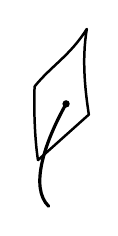
\begin{tikzpicture}[x=0.85cm,y=0.85cm,line cap=round,line join=round]
  \draw[line width=.9pt] (0.05,.69) .. controls (-.01,1.08) and (-.01,1.60) .. (.00,1.79)
    .. controls (.25,2.10) and (.53,2.25) .. (.78,2.65)
    .. controls (.70,2.18) and (.76,1.70) .. (.81,1.37)
    -- (.05,.69);
  \draw[line width=1.15pt] (.21,0) .. controls (-.08,.28) and (.15,.96) .. (.47,1.53);
  \fill (.47,1.53) circle (.055);
\end{tikzpicture}}
% archive sheet number: 2
\scanpage{4}
$X$ de type fini sur $Y$. On dit que $X$ est \unsure{monique|morique|monogène} sur $Y$ si

(i) les fibres de $X$ sur les $y\in Y$ sont \deleted{\unsure{toutes}} \unsure{ult\textsuperscript{t}|ab\textsuperscript{t}|rel\textsuperscript{t}} irréductibles

\inserted{alors la fonction $y\to\varphi(y)={}$\unsure{p\textsuperscript{t} gén.|p\textsuperscript{t} génér.} de $f^{-1}(y)$, est continue ssi $X\to Y$ est ouvert}

(ii) la fonction $\varphi$ est \unsure{la \uline{même}|\uline{bornée}}.

Une application $\varphi:Y\to X$ est dite \unsure{monisante|monisente|monogène} s'il existe un ouvert $U$ de $X$ qui est \inserted{\unsure{universell\textsuperscript{mt}|universellement}} monique sur $Y$,
\inserted{(i.e. $U$ \unsure{univ\textsuperscript{t}|universellement} ouvert sur $Y$)} tel que pour \deleted{\unsure{tout}} $y\in Y$,
$\varphi(y)$ soit le point générique de $U\cap f^{-1}(y)$. [Si $Y$ est noethérien, il revient au $=$ de dire : (i) Pour \deleted{\unsure{tout}} $y\in Y$,
$\varphi(y)$ est le p\textsuperscript{t} générique d'une composante \unsure{relativem\textsuperscript{t}|rel\textsuperscript{t}} irréductible de $f^{-1}(y)$ (ii) Si $y\in\overline{y'}$,
\deleted{\unsure{alors $\varphi(y')$ est l'unique} et \unsure{si} $x'\in f^{-1}(y')$ est \unsure{un point de} $f^{-1}(\unsure{y'|y})$ qui \unsure{générise} $\varphi(y)$ (iii) $\varphi$ \unsure{continue} tel que $\varphi(y)\in\overline{x'}$, alors $x'=\varphi(y')$.} \deleted{\unsure{iii}.} $\unsure{U|u}\to Y$ est \unsure{univ\textsuperscript{t}} ouvert.]
% slanted
\margin{\uline{Lemme} $\varphi$ \unsure{satisfaisant} (i) et (ii) implique l'existence de $U$ satisfaisant \unsure{(i)|(ii)}}
% slanted
\margin{C'est une propriété \uline{locale}.}

Si $\varphi:Y\to X$ est monisante, alors pour tout changement de base $Y'\to Y$, l'application associée $\varphi':Y'\to X'$ [définie de façon évidente] est monisante. Ainsi, l'ens
$F(X'/Y')$ des sections monisantes de $X'/Y'$ est un foncteur contravariant en $Y'$. Est-il représentable ??

Si oui, le \unsure{problème|préschéma} des modules $M$ sur $Y$ est nécessairement étale de type fini sur $Y$ [mais pas néc. séparé sur $Y$]

Soit $M$ \uline{étale} de type fini sur $Y$, et $\varphi_M$ une \deleted{section} application monisante pour $X\times_Y M\,/\,M$, qui ait la propriété suivante : Pour \deleted{tt} $y\in Y$ et une extension alg. close $\Omega$ de $k(y)$, l'application $M(\Omega)\to{}$ ens des composantes irréductibles de $X\otimes_y\Omega$ est \uline{bijective}. Alors $(M,\varphi_M)$ représente le foncteur $F$.
% slanted
\margin{\uline{\unsure{Car|Cor}} les \deleted{\unsure{pts}} \inserted{\uline{\unsure{éléments|étl\textsuperscript{mts}}}} de $M$ correspondent aux composantes irréductibles des fibres de $X\to Y$}
% archive sheet number: 3
\scanpage{5}
[On est \unsure{amené|ramené} à prouver ceci : Soit $\psi:Y\to M$ une application telle que (i) pour \deleted{tt} $y\in Y$, $k(\psi(y))=k(y)$, i.e. $\psi(y)$ est rationnel sur $k(y)$ (ii) l'application correspondante $\varphi:Y'\to X'$, \deleted{\unsure{est une}} faisant correspondre à tout $y\in Y'$ la composante \unsure{ult.|rel\textsuperscript{t}} irréd. de $f^{-1}(y)$ correspondant à \deleted{$k(y)$} $\psi(y)$, est \unsure{monisante|monisente|monogène}. -- Alors, \deleted{\unsure{que c'est une}} $\psi(Y)$ est \deleted{à la fois} ouvert. \deleted{et fermé, \unsure{et} $\psi(Y)\to Y$ est} donc $\psi$ provient d'une section de $M$ sur $Y$]~; sous cette forme, c'est évident, grâce à la condition de continuité mise \unsure{dans|ds} la définition de ``monisant'']

\uline{Conséquence} Si le Pb des modules a une solution pour $X\times_Y\operatorname{Spec}(\mathcal O_y)$ \inserted{sur $\operatorname{Spec}(\mathcal O_y)$}, \deleted{\unsure{elle a une}} il existe un ouvert $U\ni y$ tel que le Pb des modules ait une solution pour $X|U\,/\,U$.

Cela nous ramène, pour l'existence, au cas où \deleted{$X$} $Y=\operatorname{Spec}(A)$, $A$ local. \inserted{[Car \deleted{\unsure{tt}} alors supposons \unsure{$\dim Y=n<+\infty$}]} D'ailleurs, grâce à la descente des morphismes étales, on est ramené au cas où $A$ est \uline{complet},
% slanted
\margin{? descente des morphismes étales dans le cas non séparé \deleted{\unsure{finis}} ???}
et on peut $=$ supposer que la fibre $f^{-1}(y_0)$ de son point fermé se décompose en composantes \uline{ult\textsuperscript{t}} irréductibles.
% archive sheet number: 4
\scanpage{6}
\diagram{\begin{tikzcd}[ampersand replacement=\&,column sep=small,row sep=small]
 \& X\arrow[d,"f"] \&\\
 \& Y=\operatorname{Spec}(A) \&\\
 y\ \text{fermé} \& \& \eta
\end{tikzcd}}
[\uline{strictement}] universellement ouvert, de type fini

$A$ local noethérien \uline{complet}, $f^{-1}(y)$ \inserted{\unsure{ult\textsuperscript{t}|rel\textsuperscript{t}|N.B.}} irréductible

(i) Supposons que \deleted{$f^{-1}(y)$ soit \unsure{ult}} pour $\eta$ générisation convenable de $y$, il y ait \uline{deux} \uline{élts} \uline{distincts} de $E_{X/Y}(\eta)$ qui générisent $x$. En vertu du \uline{lemme} \inserted{a)}, on trouve la $=$ situation, \deleted{avec} par \unsure{changem\textsuperscript{t}} de base $Y'$,
avec \deleted{\unsure{un ann}} $Y'=\operatorname{Spec}(V)$, $V$ anneau de valuation discrète (à corps résiduel alg. clos si on veut, et alors les \deleted{\unsure{fibres}} \inserted{composantes} de $f^{-1}(\eta')$ \uline{ult\textsuperscript{t}} irréductibles), c'est donc qu'il y a \unsure{croisement|croissement|coïncidence} de composantes des fibres géométriques en $f^{-1}(y)$ i.e. en $x$. Supposons que ceci soit exclu.
% slanted
\margin{``\uline{strictement}'' \unsure{univ\textsuperscript{t}} ouvert est utilisé \unsure{seulement|seulem\textsuperscript{t}} dans (i) pour noter que s'il y a \unsure{collapsage|collapse} de fibres \deleted{\unsure{géométriques}} sur $A$, il y en a aussi sur un anneau de valuation discrète --- autrement, on ne s'en sert pas}

(ii) Soit $\xi\in E_{\unsure{\alpha|X}/Y}(\eta)$ tel que $x\in\overline\eta$ [existe, car $f$ est \unsure{univ\textsuperscript{t}} ouvert] je dis que $\overline\xi$ est \uline{ult} irréductible. \deleted{\unsure{On a en}} En effet, on peut supposer $A$ intègre, $\eta$ le p\textsuperscript{t} générique de $Y$. Faisant une extension finie \inserted{séparable} $K'$ sur $K$, \inserted{\unsure{où|rendant} $f^{-1}(\eta)\otimes_K\unsure{K'|K^i}$ décomposé}, et normalisant $A$ dedans, d'où un $A'$ fini sur $A$, on note que $A'$ est \uline{local} (car $A$ local complet). Utilisant le lemme b), \deleted{\unsure{on}} \inserted{et le fait que $f^{-1}(y)$ est \uline{ult\textsuperscript{t} irréductible}, on} trouve qu'on serait dans le cas a), absurde.

On a donc trouvé une application $\varphi:Y\to X$, associant à tout $\eta\in Y$ l'unique \inserted{p\textsuperscript{t}} \deleted{composante irréd.} $\xi$ $\in$ $E_{X/Y}(\unsure{y|\eta})$ tel que $x\in\overline\xi$, et ce $\xi$ est \unsure{ult\textsuperscript{t}|rel\textsuperscript{t}} irréd. Les conditions (i) et (ii) pour une application \unsure{monisante|monisente|monogène} sont satisfaites. Il existe donc un \uline{ouvert} $U$ de $X$ tel que \deleted{pour \unsure{tt}} $U\supset\varphi(Y)$, les fibres de $U$ sur $Y$ \unsure{ét\textsuperscript{t}|étant} ult\textsuperscript{t} irréductibles.
% archive sheet number: 5
\scanpage{7}
Reste à vérifier que $\varphi$ est \uline{continue}, \deleted{i.e. que l'image inverse par $\varphi$ d'un ouvert est un ouvert. C'est vrai sur $U=Y-y$ par hyp. de récurrence [car alors $X|U$ a une solution de modules pour} et on sait que cel. provient du fait que $X\to Y$ est \deleted{\unsure{univers\textsuperscript{t}}} ouvert.

\deleted{\uline{On obtient} ainsi}

Si on ne suppose plus $f^{-1}(y)$ irréductible, \inserted{mais ses composantes irréd. ult irréd.} on \unsure{trouve|trouver} par la méthode précédente \deleted{\unsure{on voit}} \inserted{qu'il existe $r$} fonctions \unsure{monisantes|monisentes} $\varphi_i$ $(1\leq i\leq r)$ \deleted{pour} de $X/Y$, \deleted{\unsure{correspondant} \unsure{qui sont les seules fonctions}} une pour chaque comp. de $f^{-1}(y)$. Soit \deleted{\unsure{$=$}} $Y_i=Y$ $(i=1,\unsure{--|\ldots,n})$, et $Y'_i={}$\deleted{\unsure{$X$}}$(Y-y)$, \deleted{\unsure{les}} Soit \deleted{\unsure{$X$}} enfin $M'$ la solution des modules pour $X'=X|Y'$,
% slanted
\margin{``hyp. de récurrence''}
alors les \deleted{\unsure{$X_i$}} $\varphi_i:Y'\to X$ correspondent à des sections $\varphi'_i$ de $M'/Y'$, donc à des ouverts $M'_i$ de $M'$ isomorphes aux $Y'_i$.

Recollons \deleted{les} $M'$ et les $Y'_i$ \unsure{par} \deleted{\unsure{le}} $Y'_i\to M'_i$. On trouve un préschéma $M$ \deleted{sur} quasi fini et étale sur $Y$. L'application structurale $\psi':M'\to X'\times_{Y'}M'=X\unsure{\times}{}_YM'$ et les $\varphi_i:\unsure{Y_i|X_i}\to X\inserted{=Y_i\times_Y X}$ définissent \deleted{\unsure{$\varphi$}} $\psi:M\to X\times_Y M$ qui sera une application monisante (caractère local d'une \unsure{apl.} monisante) et \unsure{sera} une solution du Pb des modules pour $X,Y$.
% archive sheet number: 6
\scanpage{8}
On a démontré le

\uline{Lemme} Soit $X$ de type fini sur $Y=\operatorname{Spec}(A)$\inserted{$y$ le p\textsuperscript{t} fermé, $Y'=Y-y$, $X'=X|Y'$}, (i) $A$ anneau local complet (ii) \deleted{$f^{-1}(y)$} Les comp. irréductibles de $f^{-1}(y)$ sont ult\textsuperscript{t} irréductibles (iii) $X$ est universellt ouvert sur $Y$ (iv) \deleted{La solution} Il existe sur $Y'=Y-y$ un \unsure{$Y$-|$Y'$-}préschéma étale \deleted{pour} modulaire pour la \deleted{\unsure{distinction des|disparition des}} \inserted{\unsure{représ.|corresp.|supp.} des} composantes \inserted{ult\textsuperscript{t}} irréductibles de $X'/Y'$

(v) Il n'y a pas de \unsure{collapsage|collapsages|recollements} ($=$ \unsure{crois\textsuperscript{mt}|croisement|coordination}) des composantes irréductibles relatives \unsure{des|de} fibres en une $=$ composante de $f^{-1}(y)$, après \inserted{n'importe quelle} extension finie de la base. \uline{Alors} il \inserted{existe} \deleted{\unsure{solution}} $Y$-préschéma \deleted{modulaire} étale $M$ modulaire pour la \unsure{représ.|corresp.|rep.} des comp. ult\textsuperscript{t} irréd. de $X/Y$.

\uline{Corollaire} \deleted{\unsure{On a}} Supposons que \inserted{$M'/Y'$ soit séparé et qu'}il n'y ait pas de \unsure{!} \deleted{\unsure{danger}} anneau de valuation discrète \deleted{\unsure{$V_1$}}$A_1$ et un hom local $A\to\deleted{\unsure{V}}A_{\unsure{1|0}}$, tel que une composante relative de $X\times_Y Y_1$ sur $\eta_1$ (p\textsuperscript{t} générique) \deleted{\unsure{en deux|soit}} \inserted{se spécialise en} \uline{deux} distinctes \deleted{\unsure{en}} $y_1$. Alors $M/Y$ est séparé.

On a \unsure{mainten\textsuperscript{ant}|maintenant} \unsure{tout} ce qu'il faut pour prouver le
% archive sheet number: 7
\scanpage{9}
\uline{Théorème} $X$ \deleted{univ. ouvert} de type fini sur $Y$. On suppose que \deleted{\unsure{en $x$ p\textsuperscript{t}}} pour \deleted{tt} p\textsuperscript{t} générique $x$ d'une \inserted{comp. d'une} fibre $f^{-1}(y)$, il existe un voisinage ouvert qui soit univ. ouvert \inserted{et qu. fini} sur un $Y[t_1,\ldots,t_n]$. (condition vérifiée p. ex. si $X$ est plat sur $Y$ en \deleted{\unsure{un}} \inserted{un tel} $x$). Pour qu'il existe un $M$ \uline{étale} et \uline{séparé} sur $Y$, \deleted{qui soit} modulaire pour les composantes irréductibles relative\inserted{s} de $X/Y$, il f. et s. que pour \deleted{tout} anneau de valuation discrète $V$ sur $Y$ [qu'on peut supposer complet à corps résiduel alg. clos, et \deleted{\unsure{les}} faisant apparaître les composantes \deleted{\unsure{des}} \uline{relatives} des \uline{deux fibres}], posant $Y'=\operatorname{Spec}(V)$ et $X'=X\times_Y Y'$, $y'$ et $\eta'$ les deux p\textsuperscript{ts} fermé et gén. de $Y'$, on ait ceci :

% A curved arrow leads from (i), at the foot, to the position before (ii).
\inserted{(i) Deux composantes \inserted{abs\textsuperscript{t}} irréductibles distinctes de $f^{-1}(\unsure{\eta'|y'})$ ne peuvent spécialiser en la $=$ composante \inserted{abs\textsuperscript{t}} irréd. de $f^{-1}(\unsure{y'|\eta'})$}

(ii) Pour \deleted{\unsure{tt|toute}} \inserted{p\textsuperscript{t} gén. $\xi'$ d'une} composante irréductible \deleted{\unsure{de $X$ de $f$} \unsure{relative|relation}} \inserted{relative} $ {f'}^{-1}(\eta')$, il existe au plus un p\textsuperscript{t} générique de comp. de $ {f'}^{-1}(y')$ qui soit dans $\overline{\xi'}$ [i.e. une composante irréd. de la fibre générale $ {f'}^{-1}(\eta')$ ne peut se spécialiser en deux composantes irréductibles distinctes de la fibre spéciale]
% archive sheet number: 8
\scanpage{10}
\uline{N.B.} Cela signifie donc que \deleted{les composantes} \inserted{l'ens des} composantes irréductibles relatives de $f^{-1}(y')$ \deleted{est \unsure{contenu}} s'\uline{injecte} dans celui des composantes irréductibles \deleted{\unsure{absolues|distinctes}} \inserted{relatives} de $f^{-1}(\eta')$\inserted{\unsure{par contre|par division|qui est}}, ce n'est pas néc. surjectif. On a cependant ceci :

\uline{Cor} Pour que $M$ soit un \uline{\unsure{revêtem\textsuperscript{t}|revêt\textsuperscript{mt}|ouvert}} étale de $Y$, il f et suffit que l'on ait de plus, avec les notations précédentes :

(iii) \deleted{\unsure{Toute|Pour}} Pour \deleted{toute} \inserted{p\textsuperscript{t} gén. $\xi'$ d'une} composante irréductible relative \deleted{\unsure{$\xi$ de $\xi'$}} de $ {f'}^{-1}(\eta')$, il existe un p\textsuperscript{t} gén. $x'$ d'une comp. irréd. relative de $ {f'}^{-1}(y')$ tel que $x'\in\overline{\xi'}$.

[Cette condition n'est pas tjrs vérifiée sous la seule condition que $f:X\to Y$ soit propre, car \deleted{\unsure{si une composante}} les fibres de $\overline{\xi'}$ peuvent être de dim str. inférieure à celle des composantes de $ {f'}^{-1}(y')$ qui les contiennent. On verra que ceci n'est pas possible s'il n'y a pas de \unsure{'idéaux|idéaux} premiers immergés ---]
% archive sheet number: 9
\scanpage{11}
\deleted{\uline{\unsure{Exemple|Corollaire}}}

\uline{Remarques} 1) La condition (i) est peut être néc. et \unsure{suffisante|suffisant|suffit} pour l'existence d'un \uline{$M$} \uline{non néc. séparé} sur $Y$.

2) La condition (i) \inserted{\deleted{et (iii)}} est satisfaite si $f$ est un morphisme \uline{séparable}. Si $f$ est de plus propre, alors \inserted{(iii) est satisfait. De plus,} le nb $\unsure{\nu|v}(y)$ des composantes irréductibles relatives (non néc. déf $/\,k(y)$) est tj continue supérieurement, \inserted{Alors} \deleted{la condition} \deleted{La conjonction de (ii) et (iii) \unsure{(iii)}, est nécessairement satisfaite,} \deleted{(ii) \unsure{équiv}} équivalence entre les conditions suivantes

a) Condition (ii) plus haut de non \unsure{scindage} d'une composante ult\textsuperscript{t} irréd. par spécialisation

b) $\nu$ est \unsure{loc|donc} constante

c) $M$ existe

\deleted{Et} Alors $M$ est \uline{propre} sur $Y$.

\figure{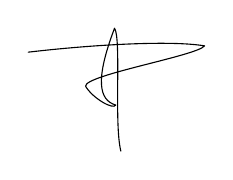
\begin{tikzpicture}[x=.8cm,y=.8cm,line join=round,line cap=round]
 \draw (.0,1.57) .. controls (1.03,1.69) and (2.26,1.76) .. (2.80,1.67)
 .. controls (2.67,1.51) and (.90,1.21) .. (.91,1.03)
 .. controls (1.02,.84) and (1.35,.65) .. (1.39,.73)
 .. controls (1.12,.81) and (1.06,1.13) .. (1.37,1.95)
 .. controls (1.48,1.79) and (1.36,.44) .. (1.47,0);
\end{tikzpicture}}
% archive sheet number: 10
\scanpage{12}
\uline{Prop} \unsure{1|1a|1\textsuperscript{o}} Soit $f:X\to Y$ un morphisme \deleted{de type fini} \deleted{\unsure{univ\textsuperscript{t} ouvert|loc.}} dont les fibres sont \deleted{\unsure{ult.}} irréductibles, Pour tt $y\in Y$, soit $\varphi(y)$ le p\textsuperscript{t} générique de $X_y$. \deleted{Pour que} \inserted{Conditions équivalentes} (i) $\varphi$ \deleted{soit} continue, \deleted{il f. et s.} \deleted{\unsure{(ii)} $y\in\overline{y'}\Rightarrow\varphi(y)\in\overline{\varphi(y')}$} \deleted{que} (ii) $f$ \deleted{soit} \uline{ouvert}. Cela implique la condition suivante, \uline{et} lui est équivalente si $Y$ est loc. noeth., $f$ de type fini :

(iii) $y\in\overline{y'}\Rightarrow\varphi(y)\in\overline{\varphi(y')}$.
\deleted{\unsure{$\Longleftrightarrow$ (ii bis)}}

\uline{Dém} \deleted{On a évidemment (i) $\Rightarrow$ (ii).} \inserted{\deleted{En effet} On a \unsure{(i)|(ii)\textsuperscript{o}} $\Longleftrightarrow$ (ii), car \deleted{\unsure{soit}} $U$ \inserted{est} un ouvert de $X$, alors $\varphi^{-1}(U)=f(U)$. De plus (ii) $\Rightarrow$ (iii) trivial.} De plus (iii) équivaut à \inserted{(iii bis) Pour tt $y,y'$ tels que $y\in\overline{y'}$, et $x$ au dessus de $y$, \deleted{tel que} il existe $x'$ au dessus de $y'$ tel que $x\in\overline{x'}$.}

En effet, \deleted{on peut supposer} (ii) $\Rightarrow$ (ii bis), car on prend $x'=\varphi(y')$, et on a $x\in\overline{\varphi(y)}$ et $\varphi(y)\in\overline{\varphi(y')}$ d'où $x\in\overline{\varphi(y')}$. On a (ii bis) $\Rightarrow$ (ii), car \deleted{il existe} si $y\in\overline{y'}$, il existe $x'$ sur $y'$ tel que $\varphi(y)\in\overline{x'}$, et comme $x'\in\overline{\varphi(y')}$, on aura $\varphi(y)\in\overline{\varphi(y')}$.

Or on sait par ailleurs que \inserted{si $Y$ loc. nth, $f$ de type fini, alors} \deleted{\unsure{(ii bis)}} \inserted{(iii bis)} $\Rightarrow$ (ii) \deleted{\unsure{donc On}} (grâce à l'hyp. \unsure{neth.}) Donc (i) $\Rightarrow$ (ii) $\Longleftrightarrow$ (ii bis) $\Longleftrightarrow$ (iii)

\uline{Déf} 2 On dit alors que $f$ est \uline{\unsure{monique|monigue|monogène}}. Définition de Universellement monique.

\uline{Déf\textsuperscript{on}} 3 Une \deleted{morphisme application} \inserted{section \unsure{ensembliste}} $\varphi:Y\to X$ est dite \uline{section} \uline{\unsure{monisante|moniquante|monigante|monogène}} si il existe un ouvert $U$ de $X$, universellement monique sur $Y$, tel que $\varphi$ soit la fonction $\varphi_{U/Y}$.
% archive sheet number: 11
\scanpage{13}
\deleted{\unsure{Si}} Alors tt \deleted{\unsure{autre}} ouvert $U'\subset U$ tel que le morphisme induit $U'\to Y$ soit \uline{surjectif}, satisfait la $=$ propriété.
% slanted
\inserted{Enfin, une réunion d'ouverts $U_i$ \deleted{\unsure{définis}} \inserted{\unsure{univ\textsuperscript{t}}} \unsure{moniques|monigues} sur $Y$ est monique sur $Y$, donc pour une section \unsure{monisante|unisante} $\varphi$, il y a un plus \unsure{gd} ouvert $U_\varphi$ \inserted{\uline{univt}} monique sur $S$ \deleted{``\unsure{contenant}'' $\varphi$ dont ce soit une \unsure{section}}.}
La propriété envisagée équivaut aussi à ceci : Pour tt $y\in Y$, $\varphi(y)$ est un p\textsuperscript{t} générique \inserted{d'une composante} de $X_y$, et il existe un \deleted{\unsure{ou}} voisinage ouvert de $\varphi(y)$ tel que \deleted{\unsure{les}} $U$ soit univ\textsuperscript{t} ouvert sur $Y$, et \deleted{\unsure{univ}} ses fibres en les pts de \unsure{plus|$\varphi(Y)$|fils}, sont ult\textsuperscript{t} irréductibles. Ce sont là des propriétés locales sur $Y$.

Si $I(X/S)$ est l'ens des sections \unsure{moniques|monogènes} de $X$ sur $S$, alors $I(X\times_S S'/S')$ est un foncteur contravariant en $S'$ de façon évidente. Est-il représentable ???

\diagram{\begin{tikzcd}[ampersand replacement=\&,column sep=small,row sep=small]
 \& X\arrow[dd] \& \& X_M\arrow[ll]\arrow[dd] \&\\
 \& \& X'\arrow[ul]\arrow[dd] \& \& X'_{M'}\arrow[ul]\arrow[ll]\\
 \unsure{k(s)|\kappa(s)}\arrow[dr,no head] \& S \& \& M\arrow[ll] \&\\
 \& \overline{k(s)} \& S'=\operatorname{Spec}(\Omega)\arrow[ul] \& \& M'\arrow[ll]\arrow[ul]\arrow[uu,"\unsure{\gamma|Y}"']
\end{tikzcd}}
% archive sheet number: 12
\scanpage{14}
\mspage{\unsure{1/|11}}
\deleted{\uline{Lemme} Soit $f:X\longrightarrow Y$ un morphisme \inserted{\uline{plat}} de type fini \deleted{\unsure{univ}} [universellement ouvert \inserted{\unsure{ou unift|ou unif$^{\mathrm t}$|en effet} \unsure{fermé}} , avec $Y$ loc$^{\mathrm t}$ noeth. \deleted{soit $y$ le point générique} Soit $y\in Y$. Alors il existe un \deleted{voisinage \inserted{ouvert}} $U$ \deleted{de $f^{-1}(y)$} \inserted{tel que $U\cap f^{-1}(y)$ soit dense dans $f^{-1}(y)$ et} tel que pour \deleted{\unsure{toute|la} \unsure{générisation de|réunion des composantes}} \inserted{générisation} $y'$ \deleted{$\unsure{\in X|\in Y}$} \inserted{de $y$} et \deleted{tout} point générique $x'$ d'une composante de $f^{-1}(y')\cap U$, il existe un point générique $x$ d'une composante de \deleted{$\unsure{\xi'|y}$} $f^{-1}(y)$ \deleted{tel que} qui soit spécialisation de $x'$.}
\margin{?}

\diagram{\begin{tikzcd}[ampersand replacement=\&]
X\arrow[d] \& X'=X\times_Y Y'\arrow[l]\arrow[d]\\
Y \& Y'\arrow[l]
\end{tikzcd}}

\[
\begin{aligned}
x_1&\in E_{X/Y}(y)\\
X_2&\in \qquad \uline{\bar\xi=\operatorname{Im}(\overline{\xi'})\ni x}
\end{aligned}
\]

\diagram{\begin{tikzcd}[ampersand replacement=\&,column sep=small]
X\arrow[d,"f"] \& x \& \xi\arrow[l] \& X'=X\times_Y Y'\arrow[d,"f'"] \& x'\arrow[d] \& \xi'\arrow[l]\arrow[d] \& X''=X\times_Y Y''\arrow[d] \& {} \& {}\\
Y \& y \& \eta\arrow[l,squiggly] \& Y' \& y' \& \eta'\arrow[l,squiggly] \& Y'' \& y'' \& \eta''\arrow[l,squiggly]
\end{tikzcd}}

\[
\uline{\text{Hyp}}\quad
\left\{\begin{aligned}
&x\in E_{X/Y}(y)\\
&\xi\in E_{X/Y}(\eta)\\
&x\in\bar\xi\\
&y'\ \text{sur}\ y\\
&\eta'\ \text{sur}\ \eta\\
&y'\in\overline{\eta'}
\end{aligned}\right.
\]

\deleted{\uline{Concl}}
\[
\begin{aligned}
&\deleted{\Gamma_{X'/Y'}(y',\eta')\longrightarrow E_{X'/Y'}(y')}\\
&\deleted{\Gamma_{X'/Y'}(y',\eta')\longrightarrow E_{X'/Y'}(\eta')}\\
&\deleted{\text{sont surjectifs}}
\end{aligned}
\]

\uline{Concl} a) Si $x'\in E_{X'/Y'}(y')$ est sur $x$, $\exists\,\xi'\in E_{X'/Y'}(\eta')$ sur $\xi$ tel que $x'\in\overline{\xi'}$.

\inserted{Si $Y'$ fini sur $Y$ et $y'$ est le seul \unsure{pt} sur $y$}
% slanted
\margin{c'est une \unsure{histoire} de \unsure{composantes} \unsure{géométriques|génériques}}

b) Si $\xi'\in E_{X'/Y'}(\eta')$ est sur $\xi$, $\exists\,x'\in E_{X'/Y'}(\eta')$ sur \deleted{$\unsure{\xi|y}$} $x$ tel que $x'\in\overline{\xi'}$.

\margin{\unsure{pour b)|pour que b)}, il faut alors que \unsure{univt ouvert|univ$^{\mathrm t}$} \unsure{p.ex.} \illegible{1} \unsure{Vérifier !}}
% archive sheet number: 13
